\chapter{SCALABLE VIDEO OBJECT SEGMENTATION \\
         WITH SPARSE SPATIOTEMPORAL TRANSFORMERS}


\section{Introduction}

Video object segmentation (VOS) involves simultaneous tracking and segmentation
of one or more objects throughout a video clip.
Our work addresses semi-supervised VOS, which conditions on one single-frame
reference annotation for each object track in a sequence.
VOS is a challenging task in which algorithms must overcome object appearance
changes, occlusion and disocclusion, as well as distinguish similar objects in
motion over time.

% NOTE(brendan): applications of VOS
Research solving these VOS challenges to create a highly performant VOS system
is important in any downstream tracking applications where pixelwise tracking
information is useful.
Tasks that can use VOS downstream include player tracking in sports analytics,
person tracking in security footage, and car and road obstacle tracking in
self-driving vehicle applications.
VOS methods are also relevant in interactive annotation of video data, where
annotator time can be used more efficiently by employing automatic video object
segmentation in an iterative annotate-predict-refine loop.
% TODO(brendan): Citation?
Furthermore, our work uses VOS as a proxy task to investigate scalable
algorithms for extracting spatiotemporal representations from video in general,
and these algorithms can be re-used for yet other video prediction tasks.

Previous methods that attempt to solve VOS can be divided into three major
categories: online finetuning, mask refinement and temporal feature
propagation.

Online finetuning, mask refinement and temporal feature propagation methods
each have inherent drawbacks.
Online finetuning methods~\cite{caelles2017one} cannot adapt to changes in
object appearance throughout a sequence.
Mask refinement and temporal feature propagation methods~\cite{ventura2019rvos}
currently in the literature are recurrent.
Due to their sequential nature, recurrent methods for VOS exhibit compounding
error over time, and are not parallelizable across a single example.

We propose a novel method for semi-supervised VOS that overcomes the drawbacks
of online finetuning and sequential methods by processing videos in a single
feedforward pass of an efficient attention-based network in which, at each
layer, each spatiotemporal feature vector simultaneously interacts with all
other feature vectors in the video.
No online finetuning is required for our method, although our method could
still benefit from online finetuning at the cost of the aforementioned runtime
penalty.
Furthermore, since our model is feedforward, we avoid the compounding error
issue inherent in recurrent methods.
Finally, SST is fully parallelizable across a single example and can therefore
take advantage of the scalability of current and future compute architectures.

% NOTE(brendan): motivation
Our method is motivated by work on Transformer architectures in language
translation, as well as by orthogonal work on correspondence matching in
computer vision.

Transformer architectures~\cite{vaswani2017attention} have shown that
end-to-end attention networks are a dominant current approach to a multitude of
text natural language processing (NLP)
tasks~\cite{devlin2019bert, dai2019transformer}, as well as speech recognition
tasks~\cite{luscher2019rwth, kim2019improved}.
% TODO(brendan): can add more references from
% https://github.com/sebastianruder/NLP-progress
Since VOS is a timeseries prediction task traditionally approached with
recurrent methods~\cite{ventura2019rvos}, and recurrent methods were succeeded
by Transformers in NLP, we hypothesized that we could achieve similar success
with Transformers in VOS as has been achieved in NLP\@.

Besides Transformers' success in NLP, we were also motivated to use attention
for VOS by the relation of attention to cross-correlation used for computing
optical flow~\cite{dosovitskiy2015flownet} and tracking~\cite{li2018high}, in
that both cross-correlation and attention use pairwise dot products of
embeddings to find matching patches of feature maps.
Methods such as FlowNet~\cite{dosovitskiy2015flownet} that use
cross-correlation to compute optical flow are relevant to semi-supervised VOS
because a perfect optical flow computation could produce a video object
segmentation by warping the reference mask throughout a video (subject to error
due to disocclusions).
However, computing perfect optical flow is difficult, particularly for the
challenging in-the-wild sequences in VOS datasets.

Our method is related to FlowNet in that we also use cross-correlation
(attention) to compute a matching of pixels in feature space.
Instead of warping an object's reference mask, we use attention to warp
object-discriminative features.
Since our method uses flow in feature space, we avoid the difficulties in
explicitly computing optical flow in pixel space.
Ultimately our method uses flow in feature space to build a spatiotemporal
object feature representation used to predict the given object's segmentation
mask over the entire video.
% TODO(brendan): refer to FlowNet paper for wording; clarify;
% compress.
Compared with warping masks with explicit flow, we also achieve efficiency
gains by instead warping compressed object features.
% TODO(brendan): numerical comparison of feature vs. mask
% dimensionality?

Applying spatiotemporal attention operators to VOS raises two challenges:
computational complexity and distinguishing foreground objects.
Na\"ive spatiotemporal attention is square in the dimensionality of the video
feature tensor, i.e.,~$O({(THW)}^2 C)$.
We resolve this computational complexity issue with sparse attention operators,
of which we compare two promising candidates.
Furthermore, we resolve the ``distinguishing foreground objects'' problem,
i.e., how to inform the model of which object to segment, by introducing an
Expand-Mask-Project operator.

% NOTE(brendan): brief summary of key results
Our work achieves an overall score of~\num{\yvosvalG} on the official
YouTube-VOS validation set, comparing favourably with prior work.
Furthermore, our method is robust to subsampling of video sequences, so that we
are able to predict future frame segmentations in constant time by sampling and
processing a fixed number of intermediate frames.
% TODO(brendan): Other results.
% Runtime? DAVIS-2017?


\subsection{Contributions}

For the first time, we apply video attention on video object segmentation, by
using sparse attention operator variants to apply Transformer models on
high-resolution videos.
We also contribute empirical evaluation of Transformer models applied to video,
as Girdhar et al.~\cite{girdhar2019video}, a work on video action recognition,
is the only prior work using Transformers on video that we are aware of.

We extend sparse attention variants to video so that they can be used for VOS.
Specifically we extend to 3D, with two spatial axes and one temporal axis,
Criss-Cross Attention~\cite{huang2018ccnet} from 2D semantic segmentation, and
Sparse Attention~\cite{child2019sparsetransformer} from 1D language
translation.
Our sparse video attention operators are not VOS specific, and could be applied
to other dense video prediction tasks.

% TODO(brendan): we evaluate the runtime and scalability of our method, and
% contrast it with RGMP.

% Ablation:
% Relative positional encodings
% Different projection operators in attention
% Sparsity variants

% We propose an object appearance model called Attention in Attention (AIA) that
% adaptively extracts a single discriminative feature vector each for a variable
% number of objects in a video.
% Our adaptively extracted object appearance models capture features that are
% discriminative even between multiple instances of the same class.

We will provide a public implementation available upon our article's acceptance.


\section{Related Work}

Our work is related to previous work in video object segmentation (VOS) and
feature matching.
We are motivated by ideas from the feature matching literature and
generalize explicit correspondence by extracting representations of transitive
correspondence between features by following connectivity patterns in 3D
activation maps.


\subsection{Video Object Segmentation}

In the VOS literature, \textbf{online finetuning}
approaches~\cite{bao2018cnn,caelles2017one,maninis2018video,voigtlaender2017online,hu2018motion,khoreva2017learning,li2018video}
do one-shot, or semi-supervised, VOS by finetuning a semantic segmentation
network on an initial frame.
A number of methods:~\cite{cheng2018fast,caelles2017one,maninis2018video,voigtlaender2017online}
performed VOS on independent frames using finetuning alone without explicitly
modelling temporal coherence.
\cite{maninis2018video} built on the original usage of this approach
in~\cite{caelles2017one} by adding instance-level semantic information,
while~\cite{voigtlaender2017online} added adaptive training during the
sequence.
\textbf{Offline} methods must use temporal information to produce future
segmentations from past frames, as done using optical flow
in~\cite{jang2017online} and~\cite{tsai2016video}.
Our method is in principle able to take advantage of online finetuning to
improve performance, and also performs competitively using offline training
alone.

Research into temporal coherence in VOS falls into two categories: those that
refine masks, and those that propagate temporal features.

\textbf{Mask refinement}
approaches~\cite{khoreva2017learning,oh2018fast,khoreva2017learning,hu2017maskrnn,jang2017online}
refine a previous mask using feedforward models.
Khoreva et al.~\cite{khoreva2017learning} implemented mask refinement by a
recurrent connection on the concatenated frame~$t-1$ output masks and frame~$t$
RGB inputs where the recurrent connection is a VGG16.
Oh et al.~\cite{oh2018fast} extended recurrent mask refinement by concatenating
the feature map from the first frame.
Yang et al.~\cite{yang2018efficient} used a spatial prior on the target
location, with channel-wise attention mechanism and meta-learning to adapt the
network to the object given in the first frame.
Bao et al.~\cite{bao2018cnn} propagated masks by approximate inference in an
MRF, with temporal dependencies based on optical flow, and spatial dependencies
using a CNN\@.
Optical flow has also been used to add motion information via jointly training
optical flow and VOS~\cite{cheng2017segflow},
while Jain et al.~\cite{jain2017fusionseg} and Hu et al.~\cite{hu2018motion}
also added motion information via optical flow.

\textbf{Temporal feature propagation}
approaches~\cite{tokmakov2017learning,xu2018youtube,hu2017maskrnn,salvador2017recurrent}
improve upon mask refinement methods by increasing the expressive power of the
mask feature representation.
At the time of writing, all temporal feature propagation methods have used RNNs
to encode and propagate spatiotemporal representations through time.
Jampani et al.~\cite{jampani2017video} also used spatiotemporal features to
forward-propagate information.

Our approach falls under the temporal feature propagation category.
We use sparse attention operators to propagate features temporally in a single
feedforward operation.

% \cite{khoreva2017lucid} used TPS for data augmentation.

% \cite{chen2018blazingly} and~\cite{hu2018videomatch} condition on a set of
% foreground and background feature vectors (?). They use KNN prediction (?).

Luiten et al.~\cite{luiten2018premvos} split the task of semi-supervised object
segmentation into two tasks.
First, Luiten et al.\ generated multiple mask proposals for each frame and then
selected and merged the masks to generate accurate and temporally consistent
masks for the video sequences.
In contrast to Luiten et al.~\cite{luiten2018premvos}, our approach is
conceptually simple, based on a single network architecture composed of
attention operators, and we perform inference in a single end-to-end forward
pass.

Voigtlaender et al.\ proposed FEELVOS~\cite{feelvos2019} as a simple and fast
method for solving the VOS problem.
Unlike most other VOS methods, Voigtlaender et al.\ trained FEELVOS end-to-end
using a pixel-wise embedding, along with global and local matching mechanisms
using the reference and previous frames to generate the masks for the video
sequence.
Our work shares similarities with Voigtlaender et al.'s~\cite{feelvos2019} in
that both methods are end-to-end trainable and conceptually simple.
Our method has the added advantages of simultaneously extracting features from
multiple frames using attention, and using positional encodings to learn
spatiotemporal position-aware representations.

Johnander et al.~\cite{johnander2019agenerative} used a Gaussian Mixture Model
representation of foreground and background appearance to propagate appearance
information forward through a video sequence.
Appearance models are complementary to our method and we show that combining
appearance models with SST performs better than either method individually.

% No online finetuning:~\cite{jang2017online}, \cite{tsai2016video} both use
% optical flow with refinement.
% \cite{li2018video} combined optical flow with an object proposal network using
% bidirectional mask propagation and target reidentification.
% \cite{cheng2018fast} track object parts and refine them with a similarity-based
% scoring function based on the reference frame.

% A generative
% \cite{johnander2019agenerative} used a Gaussian Mixture Model representation of
% foreground and background appearance to propagate appearance information
% forward through a video sequence.
% They get a best mIoU of~$67.2\%$ on DAVIS-2017.
% They get~$66.9\%$ and~$61.2\%$ mIoU on seen and unseen classes, respectively,
% on YouTube-VOS (overall mIoU~$66.0\%$).

% % RVOS
% \cite{ventura2019rvos} they use a spatiotemporal
% ConvLSTM~\cite{shi2015convolutional} to learn one- and zero-shot VOS end-to-end
% without finetuning or additional data (e.g., object proposals).
% On YouTube-VOS one-shot they get~$63.1\%$ and~$44.5\%$ mIoU on seen and unseen
% classes, respectively.
% On DAVIS-2017 one-shot they get~$48.0\%$ mIoU ($J$), and~$52.6\%$ contour
% accuracy ($F$).

% Full-frame~\cite{maninis2018video, voigtlaender2017online} vs. single
% object~\cite{xu2018youtube}.

% \cite{ren2017endtoend, romeraparedes2016recurrent} do instance segmentation by
% predicting a sequence of masks (i.e., spatial recurrence on the current frame).

% \cite{ren2017endtoend, ventura2019rvos} use a soft IoU cost function for
% bipartite matching using the Hungarian algorithm.

% VOS using Space-Time Memory Networks
% \cite{oh2019video}

% \cite{caelles2017one, yoon2017pixellevel, hu2018videomatch} all condition on
% the reference frame mask to predict future segmentations,
% while~\cite{oh2018fast, yang2018efficient} also utilize the previous frame.
% Our method, like~\cite{oh2019video}, is able to combine information from any
% subset of the entire sequence history.


% \subsection{Feature Matching (Budget: 0.5--1 pages)}

% Our work builds on the feature matching literature in the calculation of our
% correspondence scoremap.

% In~\cite{rocco2017convolutional} the authors use normalized correlation to
% regress the parametric deformation model.
% We employ a similar normalized correlation similarity measure, but to define an
% attention scoremap that we use to rank object proposals and merge semantic
% segmentation masks produced by separate, framewise models.

% In~\cite{rocco2018endtoend} the authors extend~\cite{rocco2017convolutional} to
% paired data for which groundtruth keypoint correspondences are unknown, by
% maximizing a soft-inlier count that is learned end-to-end with feature
% extraction and a geometric transformation regressor.

% The authors of~\cite{wang2019learning} use the cycle-consistency of time as a
% learning signal for self-supervised training of object tracking feature
% representations.

% In~\cite{ham2016proposal} the authors use sets of object proposals to predict
% region correspondences, which are then used to create dense flow fields.
% Our work is similar in that both works match per-frame object proposals between
% pairs of images, however~\cite{ham2016proposal} focused on semantic flow, while
% we use these correspondences for the downstream task of video object
% segmentation.
% Furthermore, our object proposal and matching methods differ from the
% methodology in~\cite{ham2016proposal}.

% Still TODO for Related Work: skim CVPR 2019, ICCV 2019 paper lists for VOS
% papers.


\section{Method}

We first present a high level view of our method's architecture, before
describing implementation details of our ``grid'' and ``strided'' sparse
attention modules for VOS\@.


\subsection{Architecture}
\label{sec:architecture}

We draw parallels with the canonical text-based Transformer
architecture~\cite{vaswani2017attention} in order to motivate our architecture.
Like NLP Transformers, our architecture consists of an encoder and decoder.
Unlike the encoder of an NLP Transformer, which takes as input embeddings
extracted from a text sequence, our encoder's input consists of the frames of
the video to segment, and the reference masks of objects to segment.
% TODO(brendan): separate concept of encoder from "setup" step
% (sampling + 2D encoding).
Like NLP Transformer decoders, our decoder conditions on the output of our
encoder.
Unlike NLP Transformer decoders, which take output sequence embeddings as
input, our decoder takes as input an object representation initialized to the
encoder reference features repeated over the length of the video.

Our encoder architecture, depicted in Figure~\ref{fig:ainaencoder}, takes a
sequence of~$T$ RGB video frames as input, and produces two streams of output:
a generic video representation stream, and an object-discriminative
representation stream.
We subsample the input video
tensor~$\inputvar{} \in \real{}^{3\times T \times H\times W}$ to a fixed size
using Temporal Segment Network (TSN) sampling~\cite{wang2016temporal} during
training.
At test time we replace subsampling with an identity function.
A 2D ResNet~\cite{he2016deep} encodes input frames independently, before
splitting them into separate streams representing the video and individual
objects-to-segment.

Our encoder architecture's generic video representation stream (top right in
Figure~\ref{fig:ainaencoder}) processes the framewise 2D ResNet output features
with a sequence of self-attention layers, adding temporal context to the video
representation.

The object-discriminative feature stream (bottom right in
Figure~\ref{fig:ainaencoder}) must provide an initialization that informs the
decoder of which objects to segment, achieved by our Expand-Mask-Project
operator shown in Figure~\ref{fig:expandmaskproject}.

% TODO(brendan): replace encoder/decoder diagrams with Inkscape polished
% versions.
% Create a diagram that parallels the Vaswani et al. architecture diagram.
\begin{figure*}
\centering
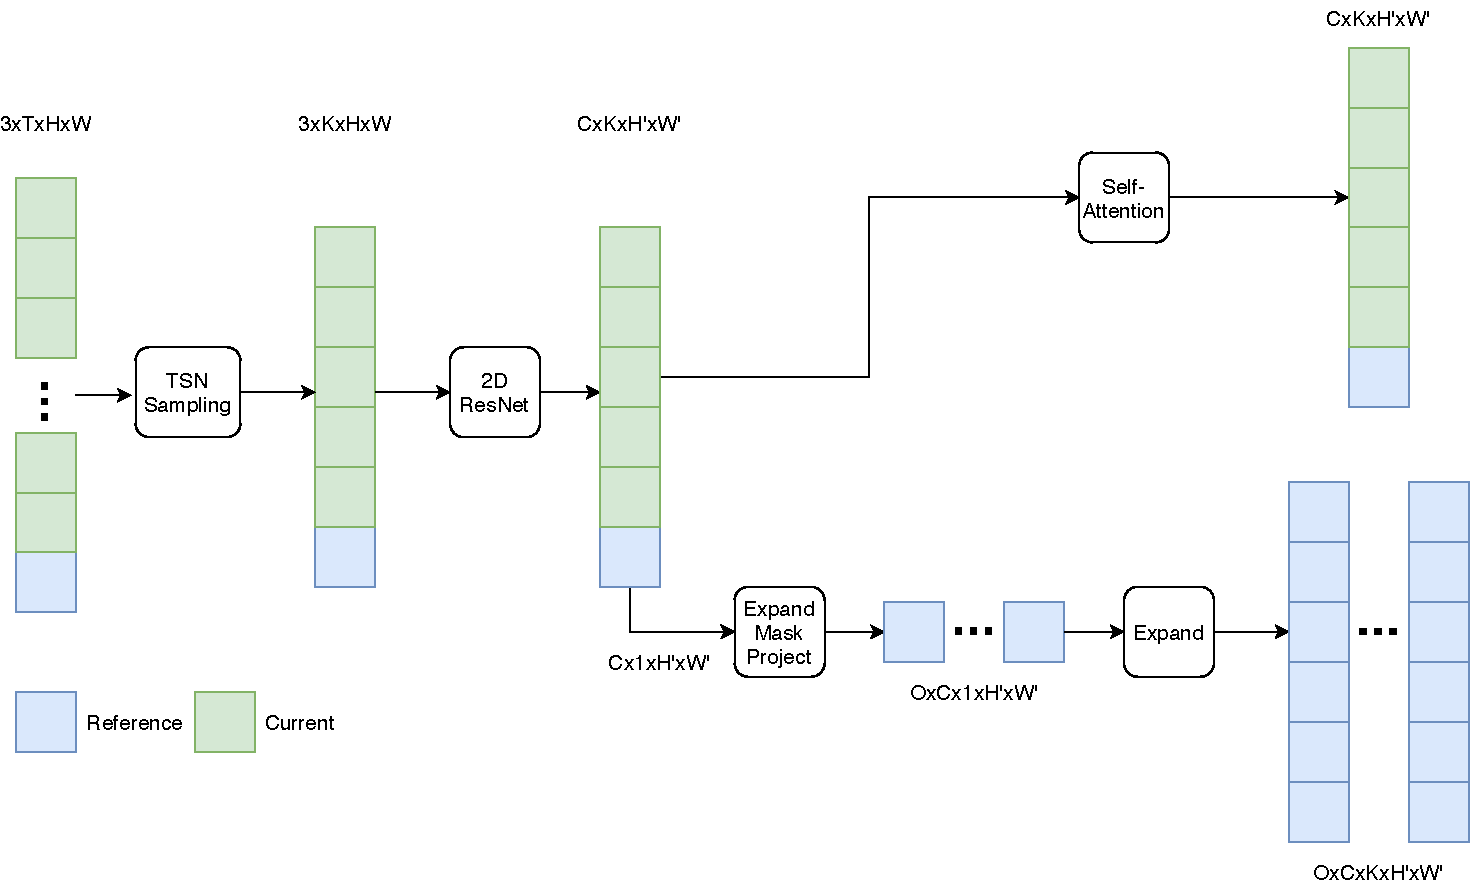
\includegraphics[width=1.0\textwidth]{Figures/aina_encoder.pdf}
\caption{SST encoder architecture.
         The input to the SST encoder is a
         video~$\in\real{}^{3\times T \times H\times W}$, where~$T$ is the
         total number of video frames.
         From left to right, the video is first subsampled (using TSN
         sampling~\cite{wang2016temporal} during training) to a fixed number of
         frames~$K$, which are processed independently by a 2D
         ResNet~\cite{he2016deep} to produce a feature tensor~$\in
         \real{}^{C\times K \times H'\times W'}$.
         The encoder then splits into two representation streams.
         The top stream encodes generic video features, and incorporates
         temporal context using a self-attention layer.
         The bottom stream encodes object-discriminative features by applying
         the Expand-Mask-Project operator to the reference features, and
         repeating the resultant feature tensor~$K$ times.
         Both streams are input to the SST decoder, described in
         Figure~\ref{fig:ainadecoder}.
         Blue indicates reference features and green indicates non-reference
         video features (best viewed in colour).}
\label{fig:ainaencoder}
\end{figure*}

The Expand-Mask-Project layer (Figure~\ref{fig:expandmaskproject}) relays to
the decoder information about whether each pixel in the feature map belongs to
an object by projecting object foreground and background to different affine
subspaces described by the parameters of affine
transformations~$T_{foreground}$ and~$T_{background}$.

To separately project object foreground and background features we use each
object's downsampled mask and inverse mask (i.e.,~$1 - M$ for binary object
mask~$M$) to extract object foreground and background features.
Foreground and background affine transformations~$T_{foreground}$
and~$T_{background}$ then project their respective extracted features to
foreground and background affine subspaces.
An elementwise addition operation then combines the projected object foreground
and background features, producing a single~$O\times C\times H'\times W'$
reference feature map, where~$O$ is the number of objects and~$C$ the number of
channels, that contains information about which pixels of the feature map
belong to which object.

Finally, the SST encoder's object-discriminative stream repeats the projected
object foreground and background features by the number of sampled frames~$K$
times along a new axis to produce an~$O\times C\times K\times H'\times W'$
output to feed into the SST decoder.

We briefly justify our choice to repeat the projected reference features across
the video.
The SST decoder gradually updates the object-discriminative features to produce
the video object segmentation.
When the SST encoder passes its object-discriminative features to the decoder,
the encoder has not yet incorporated temporal context.
Therefore, repeating the projected reference features across the video is the
encoder's best initialization for object location throughout the video based
only on the prior knowledge given in the reference frame.

\begin{figure}
\centering
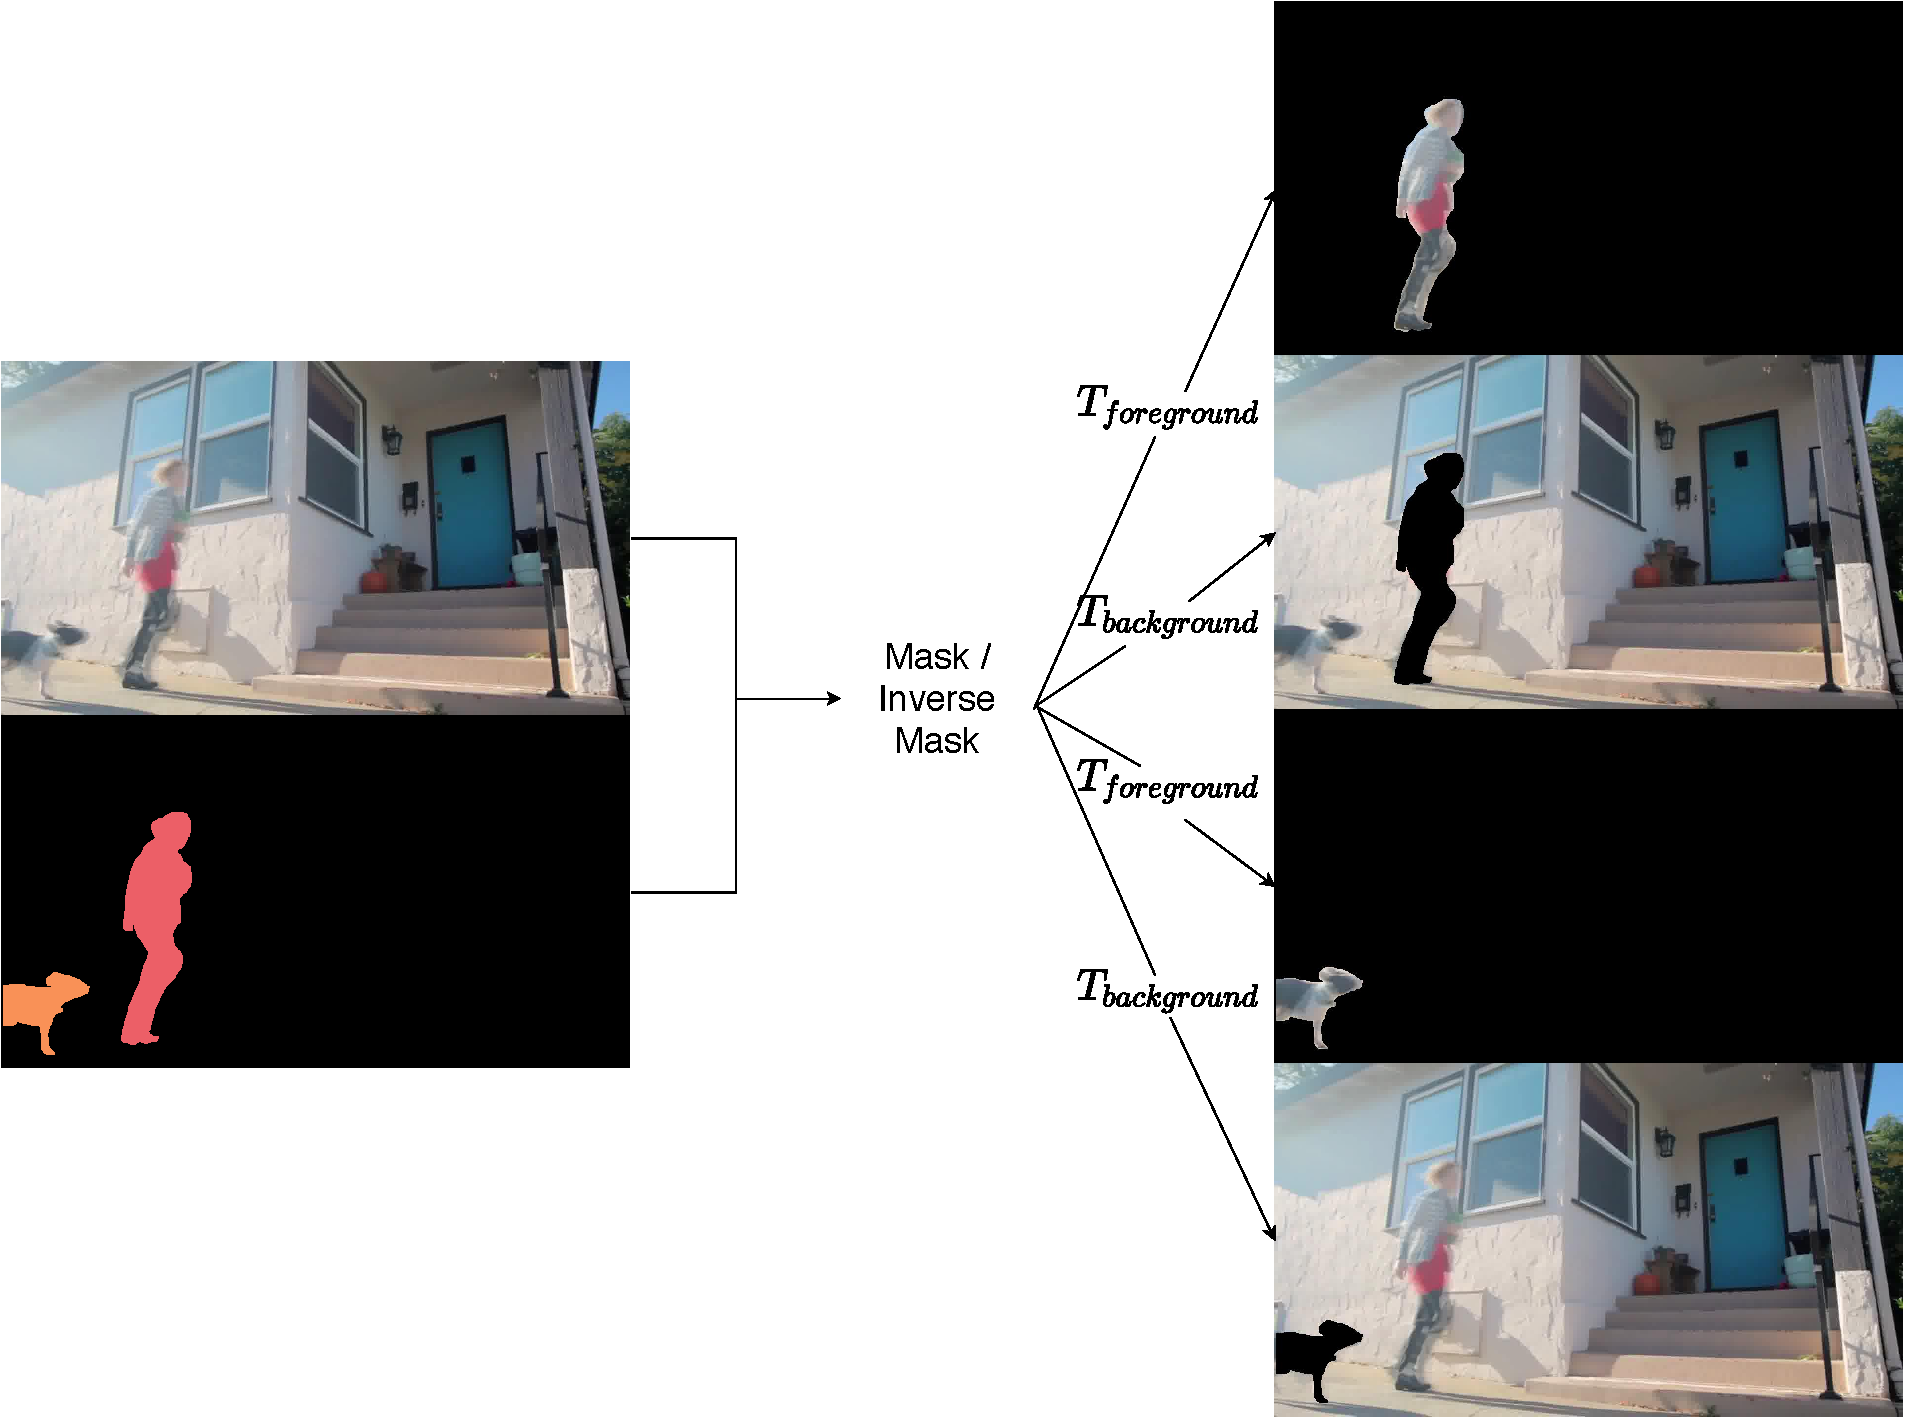
\includegraphics[width=0.9\textwidth]{Figures/expand-mask-project.pdf}
\caption{Expand-Mask-Project operator.
         We use an RGB image to visualize feature maps for clarity.
         The actual Expand-Mask-Project operator uses downsampled object masks
         and reference features processed by a 2D ResNet~\cite{he2016deep} of
         stride~\num{8}.
         % TODO(brendan): replace with feature visualization from actual model
         % (e.g., SSS visualization).
         The Expand-Mask-Project operator has three steps: \textbf{Expand},
         \textbf{Mask}, and~\textbf{Project}.
         In the~\textbf{Expand} step, we repeat the~$C\times H'\times W'$
         reference features along a new object axis to get
         an~$O\times C\times H'\times W'$ tensor, where~$O$ is the number of
         objects to segment.
         We then use each object~$o$'s foreground mask~$M_o$ and corresponding
         background mask~$1 - M_o$ in the~\textbf{Mask} step to create two
         copies of the original feature map for each object: one with only that
         object (and the background zero'ed out), and the other with only the
         background (i.e., everything besides the object, and the object
         zero'ed out).
         Finally, in the~\textbf{Project} step, we use affine
         transformations~$T_{foreground}$ and~$T_{background}$ to separately
         project each object's foreground and background to the affine
         subspaces designating foreground and background features,
         respectively.}
\label{fig:expandmaskproject}
\end{figure}

% TODO(brendan): to align this better with NLP Transformer, the
% Expand-Mask-Project operator could be moved into the decoder.
The SST encoder produces two outputs passed to the SST decoder: a generic video
feature representation~$\vidfeat{}\in\real{}^{C\times K \times H'\times W'}$,
and an initial object-discriminative video feature
representation~$\objfeat{}\in\real{}^{O\times C\times K \times H'\times W'}$.

The SST decoder, shown in Figure~\ref{fig:ainadecoder}, is a sequence of
cross-attention layers that match object-discriminative and generic video
features to warp the video object representation prior to the object's features
throughout the video.
The final layer of the SST decoder is a scoring convolution and sigmoid (at
training time) or argmax (at test time) layer that produces the video object
segmentation probability or segmentation
masks~$\outputvar{} \in \real{}^{K\times H\times W}$ from the final
object-discriminative representation.
In the case of multiple objects we have probability scoremaps
in~$\real{}^{O\times 2\times K\times H\times W}$, i.e., foreground-background
probabilities for each object for each pixel in the video, which we want to
reduce to a tensor in~$\real{}^{K\times H\times W}$ of object integer labels.
We use the ``na\"ive'' inference protocol~\cite{oh2018fast} and take, for each
pixel, the argmax over all object probabilities including the background
probability, computed as the maximum background probability over all objects.

As we elaborate on in Section~\ref{sec:sparse-attn}, each cross-attention layer
takes query~$\querytensor{}$, key~$\keytensor{}$, and value~$\valuetensor{}$
tensors as input and returns a weighted sum of~$\valuetensor{}$, where the
weight of each value at an index in~$\valuetensor{}$ increases with the dot
product of the query and key at the same index.
In the SST decoder, the role of query is played by the video representation,
while the object-discriminative representation plays the role of both key and
value, such that the function signature of each attention layer
is~$\mathtt{Attention}\big(\querytensor{} = \vidfeat{}, \keytensor{} = \objfeat{}, \valuetensor{} = \objfeat{}\big)$.
Note that in object-discriminative features~$\objfeat{}$ foreground and
background have been projected to separate affine subspaces, and we can use the
projection weights in attention to perform a lookup in either of those
subspaces to match against our video features.

From the perspective of attention as mapping a query and key-value pair, at
each step we use feature vectors from our evolving object-discriminative
representation to query the video key-value pair.
We update our previous estimate of the video object-discriminative features
with the resulting linear combination of video features from this lookup.
Intuitively, we use our prior knowledge about reference features to perform a
search in the video feature tensor to find features similar to our object.
In subsequent steps we reuse the results of previous queries to perform a
cascade of new searches for the object using our updated object feature
estimate.

% TODO(brendan): use vidfeat and objfeat notation should be in the figure.
\begin{figure*}
\centering
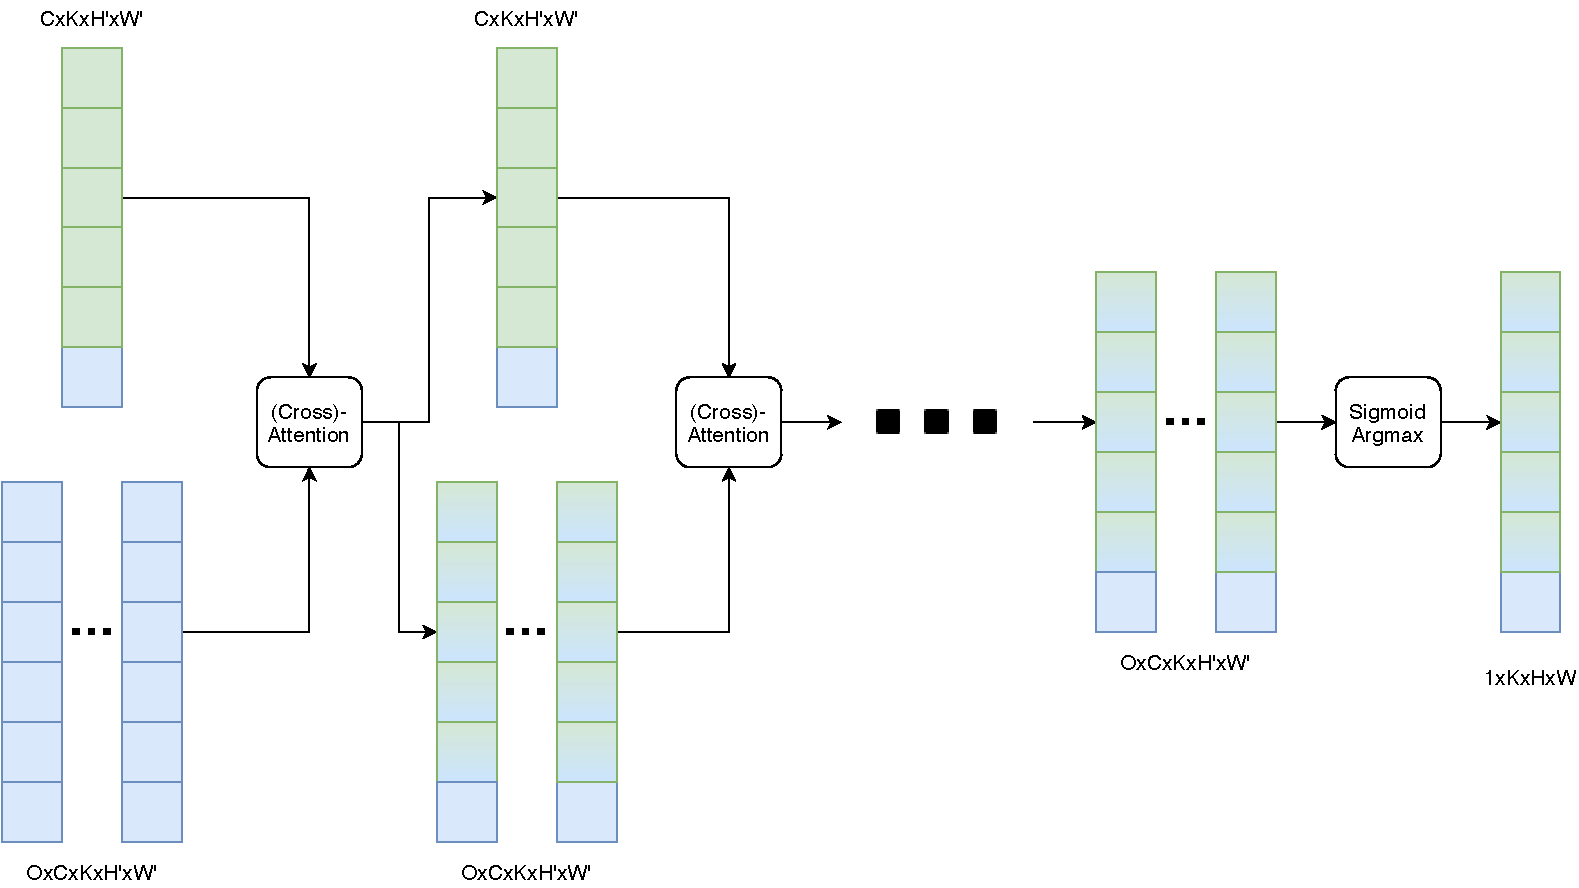
\includegraphics[width=1.0\textwidth]{Figures/aina_decoder.pdf}
\caption{SST decoder architecture.
         Decoder inputs are a generic video representation
         tensor~$\vidfeat{}\in\real{}^{C\times K \times H'\times W'}$ (top
         left, blue and green), along with object-discriminative reference
         features~$\objfeat{}\in\real{}^{O\times C\times K \times H'\times W'}$
         (bottom left, blue), where~$O$, $C$, $K$ and~$H'\times W'$ denote the
         number of objects, feature channels, subsampled video frames, and
         video spatial dimensions, respectively.
         The SST decoder is a series of cross-attention layers that warp
         reference features~$\objfeat{}$ to follow objects' movements in the
         video by matching with video features~$\vidfeat{}$.
         We use colour gradients to show that object representations after the
         decoder input are a mixture of object-specific (blue) and generic
         video (green) features, therefore this figure is best viewed in
         colour.}
\label{fig:ainadecoder}
\end{figure*}


\subsection{Sparse Attention}
\label{sec:sparse-attn}

Attention is a dense operator that allows each element of a tensor to interact
with all other elements at each attention layer.
Attention is desirable in VOS because it can capture long-range dependencies
without recurrence, and because attention can be viewed intuitively as a
cross-correlation operator that uses CNN features for
correspondence~\cite{long2014correspondence}, similar to prior work that used
matching layers for optical flow~\cite{dosovitskiy2015flownet}.

Formally, we follow~\cite{vaswani2017attention} in defining attention as

\begin{equation}
\mathtt{Attention}\big(\querytensor{}, \keytensor{}, \valuetensor{}\big) = \softmax{}\big(\querytensor{}\keytensor{}^\top\big)\valuetensor{},
\label{eqn:attndefn}
\end{equation}

\noindent where query~$\querytensor{}$, key~$\keytensor{}$, and value~$\valuetensor{}$
are all matrices in~$\real{}^{S\times C}$ for flattened spatial dimensions~$S =
THW$.
As we alluded to in Section~\ref{sec:architecture}, we use object
discriminative features~$\objfeat{}$ as query, and generic video
features~$\vidfeat{}$ as both key and value.
Intuitively we use object-discriminative features initialized by the reference
features to do a lookup in the video features in order to update our video
object features estimate.

We adapted for VOS characteristic components of the Transformer architecture as
described by Vaswani et al.~\cite{vaswani2017attention}, including multi-head
attention and positional encodings.
We compare the performance of different positional encoding schemes applied to
VOS in Section~\ref{sec:yvosablation}.
We did not normalize the softmax argument in Equation~\ref{eqn:attndefn} by the
inverse square root of channels, as we found this scaling factor hurt
performance.
The difference in impact of scaling factor between our VOS attention and
Vaswani et al.'s NLP attention could be due to our attention operator having a
comparatively low number of channels.

A computational barrier prevents na\"ively using Equation~\ref{eqn:attndefn} to
perform our desired lookup of video features~$\vidfeat{}$ using
object-discriminative features~$\objfeat{}$.
The attention operation given in Equation~\ref{eqn:attndefn} is~$O({(THW)}^2
C)$, which poses a problem for video object segmentation since for dense
prediction tasks such as segmentation, model performance tends to improve with
greater input resolution~\cite{zhao2017icnet}.
As an illustration of the infeasibility of using na\"ive attention for VOS,
consider that a single layer of attention on a~\num{16} frame video with
a~$64\times 64$ feature map with~\num{32} channels would cost more
than~\num{137} billion FLOPs, far more than the most computationally expensive
CNNs in the literature at the time of writing~\cite{tan2019efficientnet}.

We used two different sparse attention methods to make our attention operator
computationally tractable at our desired framerate and resolution.


\subsubsection{Grid Attention}

We adapted our first sparse attention operator from Huang et al., who also
noted the computational complexity issue when applying attention for semantic
segmentation~\cite{huang2018ccnet}, although in VOS the issue is exasperated
further by the addition of the time dimension.
We refer to this operator as grid attention since we have generalized it from
two to three dimensions, where the moniker criss-cross attention is no longer
fitting.

At each layer of grid attention, each pixel of the video feature activation
aggregates information from other pixels along its~$X$,~$Y$, and~$T$ axes
independently.
Each pixel interacts once with every other pixel in the video feature
activation tensor that shares at least two of its~$X$,~$Y$, and~$T$
coordinates.
Formally, for query~$\querytensor{}$, key~$\keytensor{}$, and
value~$\valuetensor{}$ tensors all in~$\real{}^{C\times T\times H\times W}$, we
define our~$\mathtt{GridAttention}$ operator as

\begin{equation}
\mathtt{GridAttention}{\big(\querytensor{}, \keytensor{}, \valuetensor{})} = \Phi\big(\Omega\big(\querytensor{}, \keytensor{}\big), \valuetensor{}\big),
\label{eqn:gridattndefn}
\end{equation}

\noindent where~$\Phi$ and~$\Omega$ are the 3D generalizations of
the~\textbf{aggregation} and~\textbf{affinity} operations defined by Huang et
al.~\cite{huang2018ccnet}.

Concretely, we define affinity operator~$\Omega$ as

% TODO(brendan): introduce superscript notation instead of Psi
% function, since superscript is more compact.
\begin{equation}
        {\Omega\big(\querytensor{}, \keytensor{}\big)}_\pixel{} = \softmax{}\big(\querytensor{}_\pixel{} {\Psi\big(\keytensor{}, \pixel{}\big)}^\top\big)
\label{eqn:gridattndefn}
\end{equation}

\noindent where~$\Psi : \real{}^{S\times C} \times \real{}^3 \rightarrow \real{}^{(T + H + W - 2)\times C}$
returns all pixels along the horizontal, vertical, or temporal axes incident to
location~$\pixel{} \equiv (x, y, t)$.
$\Omega(\querytensor{}, \keytensor{})$ is then a matrix
in~$\real{}^{S\times (T + H + W - 2)}$ where each row contains, for a pixel in
the video feature tensor, weights of a weighted average over all pixels along
its temporal, vertical, and horizontal axes.

Aggregation operator~$\Phi$ computes for each pixel~$\pixel{}$ in the video
feature tensor a weighted average over pixels along the temporal, vertical, and
horizontal axes incident to~$\pixel{}$.
Concretely, we
define~$\Phi : \real{}^{S\times (T + H + W - 2)} \times \real{}^{S\times C} \rightarrow \real{}^{S\times C}$
as

\begin{equation}
        {\Phi\big(A, \valuetensor{}\big)}_\pixel{} =  {A_\pixel{}}^\top \Psi\big(\valuetensor{}, \pixel{}\big).
\end{equation}

Note that we implemented our grid attention operator in place, so there is no
overhead from indexing tensors by~$\pixel{}$.

\begin{figure}
\centering
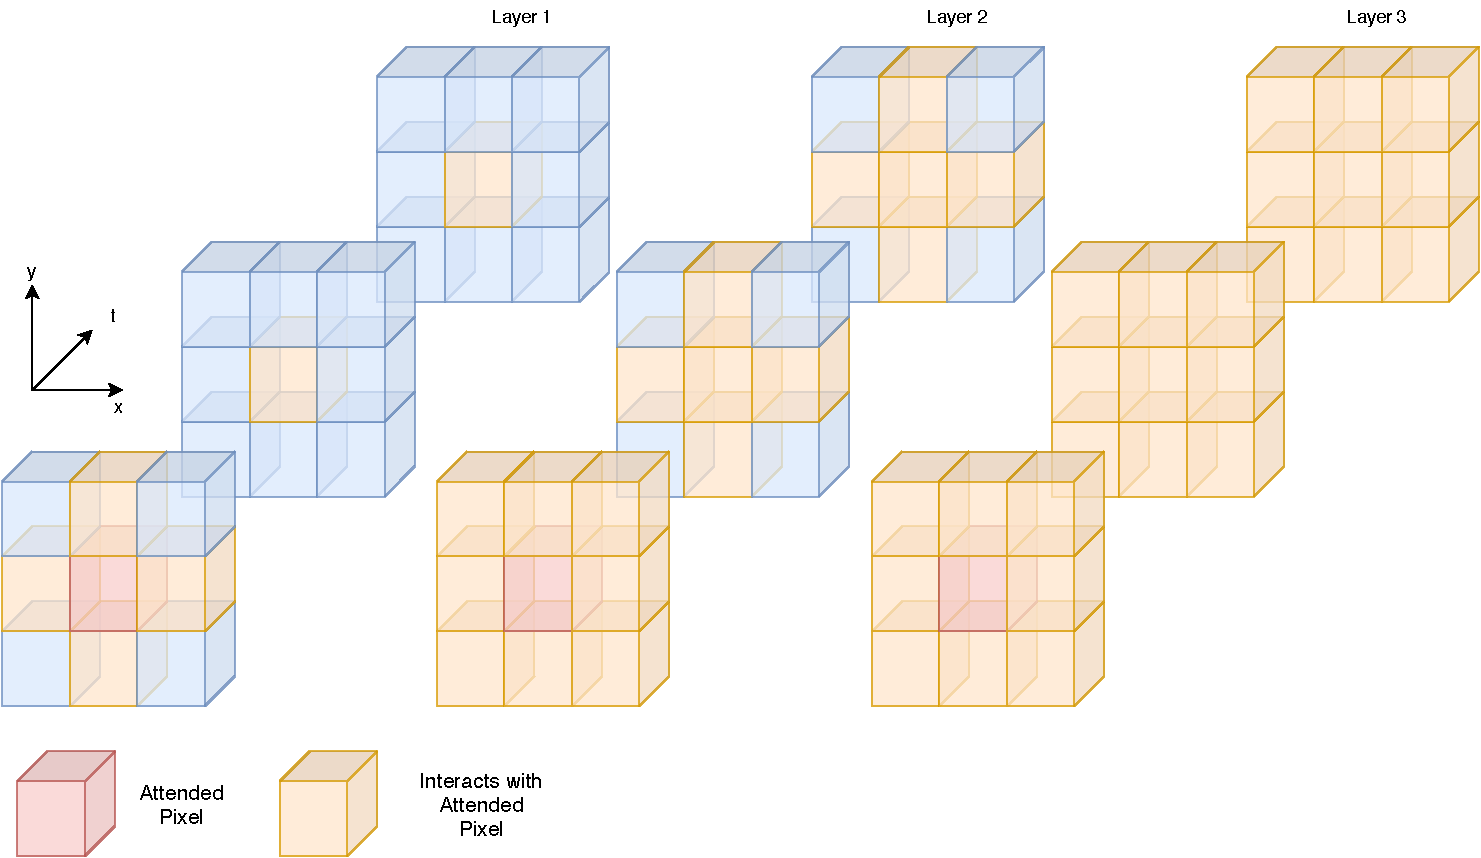
\includegraphics[width=0.9\textwidth]{Figures/gridattention.pdf}
\caption{Interaction propagation from a given pixel via grid attention.}
\label{fig:ainadecoder}
\end{figure}

In Figure~\ref{fig:ainadecoder} we illustrate how grid attention propagates
interactions from a single attended pixel to all other pixels in three
sequential layers.
The first grid attention layer propagates information to other pixels in the
same frame vertically and horizontally, and to pixels at the same spatial
location in all other frames.
The second layer propagates interactions to the entire current frame, and
vertical and horizontal axes in other frames.
Finally, the third layer propagates information to all pixels in the video
feature tensor.

% TODO(brendan): the presentation may make more sense if we use the
% reference-fg/bg features as key-value, and the video features as query.
% Then we can use the example of R = fg/bg mask to warp the mask through
% transitive correlation of video features with the reference.
To demonstrate mathematically information propagation in grid attention we
consider, for sake of clarity, a function~$\tilde{\Omega}$ that is~$\Omega$
without the softmax in Equation~\ref{eqn:gridattndefn}.
Further assume that our query is our video feature tensor, and our key and
value are both our object feature tensor,
i.e.,~$\querytensor{} = \vidfeat{}$,~$\keytensor{} = \objfeat{}$,
and~$\valuetensor{} = \objfeat{}$.
The first layer outputs, for each pixel~$\pixel{} \equiv (x, y, t)$,

\begin{equation}
\begin{split}
        \Phi{\big({\tilde{\Omega}\big(\vidfeat{}, \objfeat{}\big)}, \objfeat{}\big)}_{xyt} =
        & \sum_{i = 1}^W \big(\vidfeat{}_{xyt}^\top\objfeat{}_{iyt}\big)\objfeat{}_{iyt} + \\
        & \sum_{\substack{j = 1 \\ j \neq y}}^H \big(\vidfeat{}_{xyt}^\top \objfeat{}_{xjt}\big)\objfeat{}_{xjt} + \\
        & \sum_{\substack{k = 1 \\ k \neq t}}^T \big(\vidfeat{}_{xyt}^\top \objfeat{}_{xyk}\big)\objfeat{}_{xyk}
\end{split}
\end{equation}

We can show that composing one application of~$\Phi$ and~$\tilde{\Omega}$ with
two applications of self-attention on~$\vidfeat{}$, which we denote for brevity
as~$\Phi^3_{\tilde{\Omega}}$, produces

\begin{equation}
\begin{split}
        {\Phi^3_{\tilde{\Omega}}\big(\vidfeat{}, \objfeat{}\big)}_{xyt} =
                \sum_{i = 1}^W \sum_{j = 1}^H \sum_{k = 1}^T
                & \big(\vidfeat{}_{xyt}^\top\vidfeat{}_{iyt}\big) \\
                & \big(\vidfeat{}_{iyt}^\top \vidfeat{}_{ijt}\big) \\
                & \big(\vidfeat{}_{ijt}^\top \objfeat{}_{ijk}\big)\objfeat{}_{ijk} + \cdots,
\end{split}
\label{eqn:gridattnrouting}
\end{equation}

\noindent where~$\cdots$ represents other similar third order terms.
We show in Equation~\ref{eqn:gridattnrouting} that grid attention propagates
information along ``routes'' through the video feature tensor: for a pixel at
position~$(x, y, t)$ to interact with another pixel at an arbitrary
position~$(i, j, k)$, interactions must propagate along a ``route''  through
the video feature tensor of pairs of similar pixels.
Just as we might give travel directions through a city grid such as ``first
walk ten blocks North, then walk three blocks East'', grid attention
interactions must propagate a fixed number of pixels in the~$X$,~$Y$ and~$T$
directions, in some order, before connecting the interaction source pixel with
its target pixel.

Consider what happens if we replace the value~$\objfeat{}_{ijk}$ returned by
the inner cross-attention in Equation~\ref{eqn:gridattnrouting} with a
foreground mask value~$m_{ijk}$.
We see that the output routes reference mask values~$m_{ijk}$ over paths of
feature vectors in the video tensor~$\vidfeat{}$ that transitively correspond
to reference features~$\objfeat{}_{ijk}$.

By replacing dense attention with grid attention we reduced the computational
complexity of video attention from~$O(C{(THW)}^2)$ to~$O(C(T + H + W)THW)$,
achieving our goal of making attention tractable for video.

% TODO(brendan): unify language and notation with grid attention
%
% Path of locations


\subsubsection{Strided Attention}

We also investigated strided attention as an alternative sparse attention
method in addition to grid attention.
Drawing inspiration from Child et al.~\cite{child2019sparsetransformer}, we
propagate information by following paths of locations through sparse
connectivity patterns in our video feature tensor.
We define a connectivity
pattern~$I = \{I_{\pixel{}_0}, \dots, I_{\pixel{}_S}\}$
where~$I_\pixel{}$ is a set of coordinates~$(i, j, k)$ that index a 3D tensor.
Each layer of strided attention then returns, for each pixel~$\pixel{}$,

\begin{equation}
\mathtt{StridedAttn}{\big(\querytensor{}, \keytensor{}, \valuetensor{})}_\pixel{} = \softmax{}\big(\querytensor{}_\pixel{} \keytensor{}^\top_{I_\pixel{}}\big)\keytensor{}_{I_\pixel{}}.
\label{eqn:stridedattndefn}
\end{equation}

We define~$I_\pixel{}$ as a generalization of Child et al.'s strided attention
from 1D to 3D\@.
Our strided attention uses two different connectivity patterns~$I^1_\pixel{}$
and~$I^2_\pixel{}$ corresponding to separate, sequential heads of multihead
attention.
The first connectivity pattern~$I^1_\pixel{}$ routes to all pixels in a cube of
side-length~$h$ from~$\pixel{}$,
i.e.,~$I^1_\pixel{} = (\pixel{} + (l_x, l_y, l_z) \,:\, l_x, l_y, l_z < h)$.
The subsequent connectivity pattern~$I^1_\pixel{}$ routes to all pixels in the
video tensor that can reach~$\pixel{}$ by taking steps of size~$h$ along each
axis,
i.e.,~$I^2_\pixel{} = (\pixel{} + (l_x, l_y, l_z) \,:\, l_x, l_y, l_z \mod h = 0)$.
We choose~$h\approx \sqrt{H}$ to reduce the computational complexity by a
square root to~$O(C{(THW)}^{3/2})$ from~$O(C{(THW)}^2)$.

The relative efficiency of grid and sparse attention depends on the size
of~$T$, since we assume that~$H$ and~$W$ are comparably large and both larger
than~$T$.
During training when we subsample video sequences, sparse attention costs
about~\num{1.3} to~\num{1.4} times as many operations as grid attention, given
our training configuration where~$H, W \in \{64, 128\}$, and~$T\approx 8$.
% TODO(brendan): actual training sampling strategy for strided attention, after
% experimenting
% TODO(brendan): do Child et al. even address cross-attention?


\subsection{Appearance Model}

% Long et al.\ showed that ConvNets learn correspondence, and furthermore ConvNet
% features can align intraclass instances~\cite{long2014correspondence}.
% By using attention for VOS we leverage this correspondence property of ConvNet
% features in order to do pixelwise tracking.  However, to adapt attention to VOS
% we must extract representations that distinguish one object from another,
% whereas Long et al.\ showed that intraclass ConvNet features match so well that
% they are effective for intraclass alignment~\cite{long2014correspondence}.
% Therefore we introduce ``Attention in Attention'', an operator responsible for
% adaptively adjusting object representations to become discriminative features
% even in the presence of multiple instances of the same class.

% Our ``Attention in Attention'' (AIA) operator adaptively updates appearance
% models of each object through inter-object attention.
Johnander et al.\ showed that appearance models are effective for VOS,
particularly in generalizing to classes not seen in the training
set~\cite{johnander2019agenerative}.  Hence, following Johnander et al., we
define object appearance models as

\begin{subequations}
\begin{align}
        \objmean{} &= \frac{\sum_\pixel{}\alpha_{\pixel{}, o} x_\pixel{}}{\sum_\pixel{}\alpha_{\pixel{}, o}} \\
        \objcov{} &= \frac{\sum_\pixel{}\alpha_{\pixel{}, o} \mathrm{diag}\{{(x_p - \objmean{})}^2 + r_k\}}{\sum_\pixel{}\alpha_{\pixel{}, o}}
\end{align}
\label{eqn:appearancemodel}
\end{subequations}

\noindent where~$o$ indexes objects in the video,~$\pixel{}$ indexes pixels in the
video,~$\alpha_{\pixel{}, o} \in \{0, 1\}$ indicates whether a given
pixel~$\pixel{}$ in the reference frame belongs to object~$o$,
and~$r_k$ are model parameters.

Since~$\alpha_{\pixel{}, o}$ takes discrete values of unity inside an object,
and zero outside, in our current definition we still form object appearance
models~$(\objmean{}, \objcov{})$ independently of other objects in a video.
We hypothesize that future work on a learned component that incorporates
explicit knowledge about visual context, including both other objects and
background, into an object's appearance model would improve the ability to
extract object representations that are discriminative.

The log probability of a pixel's feature vector being generated by a given
object's appearance model forms an additional feature, which is concatenated to
the input to the self-attention block in the SST encoder.

% We use AIA to adaptively incorporate visual context into the appearance model
% defined in Equation~\ref{eqn:appearancemodel}.
% We define AIA as a dense attention operation between the appearance models of
% all objects in a video, as well as the background.
% Concretely, let~$U \in \real{}^{(O + 1)\times C}$ be the matrix of object
% appearance model means~$\objmean{}$, including the background.
% We compute an attention matrix~$A\in \real^{(O + 1)\times (O + 1)}$ as

% \begin{equation}
% A = \softmax{\big(UW_q {(UW_k)}^\top\big)}.
% \end{equation}

% Then we update each object~$o$'s appearance model~$\objmean{}$ to become a
% visual-context-aware appearance model~$\objctx{}$, defined as

% \begin{equation}
%         \objctx{} = \objmean{} + {(AUW_v)}_k.
% \end{equation}

% where~${(AUW_v)}_k$ is the~$o$th row of attention over objects, which provides
% a weighting over object means~$U$ projected by learned weights~$W_v$.

% AIA gives our appearance models the ability to incorporate visual context from
% other objects and background.
% For example, if two objects~$o$ and~$l$ have appearance models with a
% difference vector~$\bm{\mu}_k - \bm{\mu}_l \equiv \Delta$, AIA can update both
% objects to be more distinguishable so
% that~$\tilde{\bm{\mu}}_k - \tilde{\bm{\mu}}_l = \alpha\Delta$ for~$\alpha > 1$.
% In Section~\ref{sec:experiments} we demonstrate improvement from adding the AIA
% operator.


\section{Experiments and Results}
\label{sec:experiments}

We present benchmark experiment results against state-of-the-art (SOTA) methods
on the DAVIS 2016~\cite{perazzi2016abenchmark}, DAVIS
2017~\cite{ponttuset2017davis}, and YouTube-VOS~\cite{xu2018youtubevos}
datasets.
% We further analyze the effect of different sparse attention operators,
% positional encodings, and AIA operator variations through ablation studies
% using YouTube-VOS\@.
We further analyze the effect of different sparse attention operators and
positional encodings through ablation studies using YouTube-VOS\@.


\subsection{YVOS}
% YVOS comparison to SOTA

\begin{table}
\caption{Comparison with SOTA methods on YouTube-VOS~\cite{xu2018youtubevos}.
         We compute region similarity~\J{} over seen and unseen
         categories, then average those scores with contour
         accuracy~\F{} seen and unseen to get overall
         score~\G{}.
         We compute region similarity and contour accuracy as
         in~\cite{perazzi2016abenchmark}.
         We distinguish methods by those that use online finetuning (O-Ft), and
         those that do not.}
\centering
\begin{tabular}{@{}lcrrr@{}}
\toprule
Method & O-Ft & \begin{tabular}{@{}r@{}}\G{} overall \\ (\%)\end{tabular} & \begin{tabular}{@{}r@{}}\J{} seen \\ (\%)\end{tabular} & \begin{tabular}{@{}r@{}}\J{} unseen \\ (\%)\end{tabular} \\
\midrule
S2S~\cite{xu2018youtube} & \yesmark & 64.4 & 71.0 & 55.5 \\
OSVOS~\cite{caelles2017one} & \yesmark & 58.8 & 59.8 & 54.2 \\
OnAVOS~\cite{voigtlaender2017online} & \yesmark & 55.2 & 60.1 & 46.6 \\
MSK~\cite{khoreva2017learning} & \yesmark & 53.1 & 59.9 & 45.0 \\
\addlinespace[1mm]
OSMN~\cite{yang2018efficient} & \nomark & 51.2 & 60.0 & 40.6 \\
S2S~\cite{xu2018youtube} & \nomark & 57.6 & 66.7 & 48.2 \\
RGMP~\cite{oh2018fast} & \nomark & 53.8 & 59.5 & 45.2 \\
A-GAME~\cite{johnander2019agenerative} & \nomark & 66.0 & 66.9 & \textbf{61.2} \\
\textbf{SST (Grid)} & \nomark & 66.5 & 67.8 & 60.2 \\
\textbf{SST (Strided)} & \nomark & \textbf{68.1} & \textbf{69.9} & 60.8\\
\bottomrule
\end{tabular}
\label{tab:sota-yvos}
\end{table}

YouTube-VOS~\cite{xu2018youtubevos} is a large scale VOS dataset comprised
of~\num{4453} YouTube video clips spanning~\num{94} object categories.
YouTube-VOS includes an official validation set of~\num{474} videos with
heldout labels, which can be evaluated only through an evaluation server.
The YouTube-VOS validation set contains~\num{26} object categories that are
unique to the validation set, used to test the generalization capability of VOS
models to object classes unseen in the training set.
The convention is to compute region similarity~\J{} and contour accuracy~\F{}
as defined by Perazzi et al.~\cite{perazzi2016abenchmark}.
As a single metric for comparing results, it is also customary to compute
overall score~\G{} as the average of four values comprising region similarity
and contour accuracy scores for seen and unseen classes.

In Table~\ref{tab:sota-yvos} we present our model's results on YouTube-VOS
alongside previous SOTA results.
Our model (SST) performs favourably against all previous methods in overall
score~\G{}, even methods that use online finetuning (denoted by O-Ft).

Note that our unique method performs competitively against recurrent methods
that have undergone multiple research and development cycles where one method
builds on the foundation of another, for
example~\cite{johnander2019agenerative} extends~\cite{oh2018fast}, which in
turn extends~\cite{khoreva2017learning}.


\subsection{DAVIS}
% DAVIS comparison to SOTA

% TODO(brendan): runtime comparison?
\begin{table}
\caption{Comparison with SOTA methods on DAVIS2017~\cite{ponttuset2017davis}.}
\centering
\begin{tabular}{lcrrr}
\toprule
Method & O-Ft & \begin{tabular}{@{}r@{}}\JandF{} mean \\ (\%)\end{tabular} & \begin{tabular}{@{}r@{}}\J{} \\ (\%)\end{tabular} & \begin{tabular}{@{}r@{}}\F{} \\ (\%)\end{tabular} \\
\midrule
CINM~\cite{bao2018cnn} & \yesmark & 70.6 & 67.2 & 74.0 \\
OSVOS-S~\cite{maninis2018video} & \yesmark & 68.0 & 64.7 & 71.3 \\
OnAVOS~\cite{voigtlaender2017online} & \yesmark & 65.4 & 61.6 & 69.1 \\
OSVOS~\cite{caelles2017one} & \yesmark & 60.3 & 56.6 & 63.9 \\
\addlinespace[1mm]
DyeNet~\cite{li2018video} & \nomark & 69.1 & 67.3 & 71.0 \\
RGMP~\cite{oh2018fast} & \nomark & 66.7 & 64.8 & 68.6 \\
VM~\cite{hu2018videomatch} & \nomark & - & 56.5 & - \\
FAVOS~\cite{cheng2018fast} & \nomark & 58.2 & 54.6 & 61.8 \\
OSMN~\cite{yang2018efficient} & \nomark & 54.8 & 52.5 & 57.1 \\
A-GAME~\cite{johnander2019agenerative} & \nomark & 70.0 & 67.2 & 72.7 \\
\textbf{SST (Strided)} & \nomark & \davisvalG & 50.5 & 55.9 \\
\bottomrule
\end{tabular}
\label{tab:sota-davis}
\end{table}

DAVIS2017 is the latest dataset in the DAVIS initiative to promote VOS
research.
DAVIS2017 comprises 150 sequences, which include 376 separately annotated
objects~\cite{ponttuset2017davis}.

We additionally evaluate our method on DAVIS2017~\cite{ponttuset2017davis}, and
compare our results with SOTA in Table~\ref{tab:sota-davis}.
We report our DAVIS results following the traditionally used region
similarity~\J{} and contour accuracy~\F{} metrics as well as their
mean~\JandF{}.
% Our DAVIS2017 evaluation provides additional experimental evidence that SST
% method performs favourably compared with existing SOTA methods, since SST
% achieves a mean~\JandF{} score of~$\davisvalG$, whereas previous SOTA scored
% a~\JandF{} of~\num{70.6}.
According to our DAVIS2017 evaluation, SST performs relatively poorly
compared to prior work, since SST achieves a mean~\JandF{} score
of~$\davisvalG$, whereas previous SOTA scored a~\JandF{} of~\num{70.6}.
We believe that our method's performance on the DAVIS2017 validation set is
reflective of a weakness of our current formulation.
The DAVIS2017 validation set is made up of only~\num{30} sequences, and since
the DAVIS2017 evaluation is done per object, sequences with many objects are
weighed far heavier in the evaluation.
For example, a single sequence with a group of people dancing accounts for more
than~\num{10}\% of the final score.

We hypothesize that our method performs poorly on exactly the sequences that
DAVIS2017 weighs heavily in evaluation, where there are many objects of the
same class that need to be tracked in a video.
We observe that in these cases our method performs well in the initial frames,
and then our method's performance deteriorates rapidly.
SST's most common failure mode is confusing multiple objects of the same class
in medium and long temporal sequence lengths.

Long et al.\ showed that ConvNets learn correspondence, and furthermore ConvNet
features can align intraclass instances~\cite{long2014correspondence}.
By using attention for VOS we leverage this correspondence property of ConvNet
features in order to do pixelwise tracking.
However, to adapt attention to VOS we must extract representations that
distinguish one object from another, whereas Long et al.\ showed that
intraclass ConvNet features match so well that they are effective for
intraclass alignment.
We believe that the inductive bias of recurrent methods gives a temporal cue to
the VOS model to favour matching features that are spatially nearby, since
recurrent methods always propagate information from the previous frame.
Since our method currently lacks this inductive bias, our model is unable to
separate objects of the same class beyond the initial frames close to the
reference frame.
In future work we propose to inject this same ``spatial locality'' inductive
bias into SST by updating our object-discriminative and reference features
gradually with the predictions from earlier layers, instead of simply
initializing object-discriminative and reference features with the reference
frame.

We evaluate only on DAVIS2017 and not DAVIS2016~\cite{perazzi2016abenchmark}
because DAVIS2017 is strictly a more challenging superset of DAVIS2016.
Furthermore DAVIS2016 contains only single object annotations and therefore we
could make only limited evaluation of SST's ability to handle multi-object
context using DAVIS2016.
In general we consider YouTube-VOS the currently most superior benchmark for
comparing VOS algorithms due to its large size, variety, evaluation on a
heldout set using an evaluation server, as well as its unseen classes, which
are useful for evaluating generalization.


% TODO(brendan): MOTS comparison to SOTA (time permitting)


\subsection{Ablation Studies}
\label{sec:yvosablation}
% YVOS ablation studies

% \begin{table}
% \caption{Performance decay evaluation on DAVIS2017~\cite{ponttuset2017davis}.}
% \centering
% \begin{tabular}{lccr}
% \toprule
% Method & O-Ft & Recurrent & $\mathcal{D}$ \\
% \midrule
% RGMP~\cite{oh2018fast} & \nomark & \yesmark & \\
% \textbf{SST} & \nomark & \nomark & 0.21 \\
% \bottomrule
% \end{tabular}
% \label{tab:decay}
% \end{table}

We were motivated to use attention-based models for VOS due to spatiotemporal
attention's ability to incorporate temporal context without incurring a decay
in performance due to accumulating errors as is inherent to reccurent and
optical flow methods, and also noticed by Yang et al.~\cite{yang2019anchor}.
% We tested our hypothesis that SST alleviates the compounding error issue
% quantitatively on DAVIS2017 with the decay~$\mathcal{D}$ metric defined by
% Perazzi et al.~\cite{perazzi2016abenchmark}.
% In Table~\ref{tab:decay} we compare against Oh et al.'s recurrent work
% RGMP~\cite{oh2018fast}, and show that our method's performance is relatively
% robust to decay with a decay of~$\mathcal{D} = 0.21$ compared with
% RGMP's~$TODO$.
In Figure~\ref{fig:ainaocclusion} we show a qualitative example on the
YouTube-VOS validation set of SST handling foreground occlusion, where a
motorcycle entirely occludes a person for one frame then the person becomes
disoccluded in the following frame.

\begin{figure}
\centering
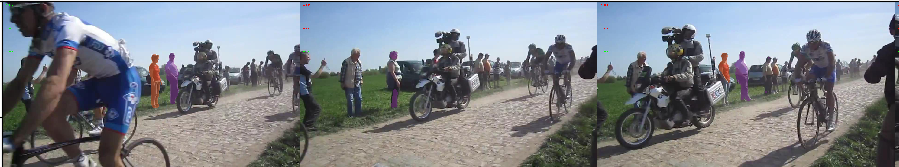
\includegraphics[width=0.9\textwidth]{Figures/aina-occlusion}
\caption{A qualitative example from YouTube-VOS validation of SST handling
         occlusion.}
\label{fig:ainaocclusion}
\end{figure}

We used YouTube-VOS to perform ablation studies on interesting components of
our method, including sparse attention operators and positional encodings.

\begin{table}
\caption{Comparison of positional encoding schemes for the ``grid'' sparse
         attention variant of video attention.}
\centering
\begin{tabular}{lr}
\toprule
Positional Encoding & Grid~\G{} \\
\midrule
None & \num{61.1}  \\
$K$ Embedding & \num{61.8} \\
$T$ Embedding & \num{60.5} \\
$T$ Sinusoidal & \num[math-rm=\mathbf]{62.6} \\
\bottomrule
\end{tabular}
\label{tab:pos-encoding}
\end{table}

In Table~\ref{tab:pos-encoding} we compare the performance of different
positional encoding schemes using the overall score~\G{} on the YouTube-VOS
validation set.
For spatial dimensions we followed Parmar et al.~\cite{parmar2019standalone} in
using learned relative positional embeddings as the encoding, following Parmar
et al.'s findings that relative are superior to absolute positional embeddings
for spatial attention.
Since we contribute an extension of attention-based models from 2D to 3D, we
focused on experimental investigation of different temporal positional
encodings.

As we described in Equation~\ref{eqn:stridedattndefn}, in sparse video
attention we propagate information through the outer product of query
tensor~$\querytensor_\pixel$ with key tensor~$\keytensor_{I_\pixel}$ indexed by
connectivity pattern~$I_\pixel$.
Adding relative positional embeddings, Equation~\ref{eqn:stridedattndefn} becomes

\begin{equation}
        \mathtt{StridedAttn}{\big(\querytensor, \keytensor, \valuetensor)}_\pixel{} = \softmax\big(\querytensor_\pixel{} \big(\keytensor^\top_{I_\pixel} + \embtensor^\top_{\tilde{I}_\pixel}\big)\big)\keytensor_{I_\pixel}
\end{equation}

\noindent where~$\tilde{I}_\pixel{} = (f(q, \pixel) : q \in I_\pixel)$
is the sequence of relative position indices for points~$q$ in
sequence~$I_\pixel$ relative to pixel~$\pixel$,
and~$f \,:\, \real^3\times \real^3 \rightarrow \real$ is a function mapping
pairs of positions to scalar indices.
For grid attention pixel~$q$ would differ along at most one of the
three spatiotemporal axes~$X, Y, T$, so the relative positional embedding for
pair~$(\pixel, q)$ would correspond to
either~$\Delta_x \equiv q_x - \pixel_x$,
$\Delta_y \equiv q_y - \pixel_y$,~or~$\Delta_t \equiv q_t - \pixel_t$.
For strided attention, the relative positional embedding would be the
concatenation of three separate embeddings corresponding
to~$\Delta_x$,~$\Delta_y$, and~$\Delta_t$.

In addition to relative positional embeddings, we also investigated sinusoidal
positional encodings for the temporal dimension, as used by Vaswani et
al.~\cite{vaswani2017attention} in Transformers for language translation.
We hypothesized that sinusoidal positional encodings would be superior to
absolute positional embeddings because of the data imbalance of absolute
temporal positions in VOS datasets, which are skewed towards lower frame
numbers.
Sinusoidal positional encodings can be interpolated or extrapolated to
generalize to underrepresented absolute frame numbers, whereas absolute
positional embeddings have no such generalization mechanism.
Furthermore, we hypothesized that sinusoidal positional encodings would be
superior to relative positional embeddings because the absolute position
information encoded in the sinusoidal representation encodes information about
a given pixel's temporal distance from the reference frame, whereas relative
positional embeddings encode no information related to distance from the
reference frame.

We present our results comparing different positional encodings in
Table~\ref{tab:pos-encoding} for both grid and strided sparse attention
variants.
The positional encoding labeled ``None'' is our baseline attention with no
positional information, while all remaining positional encodings use relative
positional embeddings for spatial dimensions~$X, Y$.
``$K$ Embedding'' and~``$T$ embedding'' refer to using relative and absolute
temporal positional embeddings, respectively, and~``$T$ sinusoidal'' refers to
using a sinusoidal temporal positional encoding.
Relative temporal positional embeddings outperformed the baseline, while
absolute temporal positional embeddings underperformed the baseline, possibly
due to the data imbalance of absolute temporal positions.
Sinusoidal temporal positional encodings performed best, which is in line with
our hypothesis that information about distance-from-reference is important in
positional encodings for VOS\@.

\begin{table}
\caption{Comparison of sparse and dense evaluation on
         YouTube-VOS~\cite{xu2018youtubevos} for both strided and grid sparse
         attention variants.}
\centering
\begin{tabular}{llr}
\toprule
Method & Evaluation & \G{} \\
\midrule
SST (Grid) & Sparse & \num{65.8} \\
SST (Grid) & Dense & \num{66.5} \\
SST (Strided) & Sparse & \num{66.7} \\
SST (Strided) & Dense & \num[math-rm=\mathbf]{68.1} \\
\bottomrule
\end{tabular}
\label{tab:evalsparse}
\end{table}

At training time we used TSN sampling~\cite{wang2016temporal} to subsample
sequences to a fixed number of frames since backpropagation constrained our
memory usage.
However at test time we do not have the same memory constraint, so we have the
ability to simultaneously predict on an entire sequence of frames at once.
In Table~\ref{tab:evalsparse} we compare the TSN and ``all frames'' test time
sampling methods, which we refer to as sparse and dense evaluation,
respectively.
We show that simultaneously attending to all frames densely produces superior
predictions for both grid and strided sparse attention variants.
We also maintain reasonable accuracy when using TSN sampling at test time to
subsample sequence, showing an advantage of our method over recurrent methods
that would have to process every preceding frame in order to predict on a given
timestep.

% TODO(brendan): grid vs. sparse discussion


\subsection{Discussion}

Our work represents the first algorithm for VOS purely based on end-to-end
attention.
Future work in attention-based models for VOS could be analogous to Transformer
models' progression on language translation tasks, where researchers
successfully applied Transformers to increasingly long sequences.
For example, Dai et al.\ combined recurrence with attention to translate
arbitrary-length sequences~\cite{dai2019transformer}, and Kitaev et al.
introduced locality-sensitive hashing instead of dot-product attention, to
reduce computational complexity from squared to~$O(N\log N)$ while using
reversible networks to model arbitrary-length sequences with constant memory
usage~\cite{kitaev2020reformer}.
In order to evaluate VOS on long sequences the VOS community would have to
overcome a dataset creation challenge, since the current benchmark dataset
YouTube-VOS contains sequences with at most~\num{36} labeled frames, sampled
at~\num{6} frames per second.
We propose that future work could use interactive and semi-automatic annotation
methods, based on the existing high-quality VOS models, to create datasets with
longer and therefore more challenging sequences.


\section{Conclusions}

We presented Sparse Spatiotemporal Transformers (SST), which constitutes the
first application of an entirely attention-based model for video object
segmentation (VOS).
We showed that SST is capable of state-of-the-art results on the benchmark VOS
dataset YouTube-VOS, attaining an overall score of~$\mathcal{G} = \yvosvalG$,
while having superior runtime scalability compared with previous state of the
art methods.
We provide code to reproduce all experiments in our work, including sparse
video-attention operator implementations, so that the community can build on
the promising idea of using attention-based models for video, in the VOS domain
and beyond.
